\documentclass[12pt]{article}
% Préambule commun à tous les documents extraits de « La Revue CAPES »
\usepackage[T1]{fontenc}
\usepackage[utf8]{inputenc}
\usepackage{lmodern}
\usepackage{amsmath,amssymb,amsthm,amsfonts,mathrsfs}
\usepackage{setspace}
\usepackage{listings}
\usepackage{pgfplots}
\pgfplotsset{compat=1.18}
\usepackage{longtable}
\usepackage{adjustbox}
\usepackage{lettrine}
\usepackage{tkz-tab}
\usepackage{changepage}
\usepackage{pdflscape}
\usepackage{graphicx}
\usepackage{tikz}
\usepackage{xcolor}
\usepackage[a4paper,top=2cm,bottom=2.5cm,left=2.5cm,right=2cm]{geometry}
\usepackage{fancyhdr}
\usepackage{draftwatermark}
\SetWatermarkText{La RevueCapes}
\SetWatermarkLightness{0.9}
\SetWatermarkScale{2}
\usepackage{hyperref}
\hypersetup{colorlinks=true,linkcolor=blue!50!black,urlcolor=blue!50!black}

\definecolor{revue}{RGB}{20,60,120}

\pagestyle{fancy}
\fancyhf{}
\renewcommand{\headrulewidth}{0.4pt}
\setlength{\headheight}{15pt}

% \entete{Matière}{Titre}{Type de document}
\newcommand{\entete}[3]{%
  \fancyhead[L]{\small\textsc{La Revue CAPES} -- #1}%
  \fancyhead[R]{\small #2}%
  \fancyfoot[C]{\thepage}%
  \thispagestyle{plain}%
  \begin{center}
    {\color{revue}\rule{\textwidth}{1.2pt}}\\[4pt]
    {\small\textsc{Concours directs CAP-CEG / CAPES -- Burkina Faso}}\\[6pt]
    {\LARGE\bfseries\color{revue} #2}\\[6pt]
    {\large\itshape #1 -- #3}\\[2pt]
    {\color{revue}\rule{\textwidth}{1.2pt}}
  \end{center}
  \vspace{0.5cm}%
}

% Encadré pour les remarques ajoutées dans les corrigés
\newcommand{\remarque}[1]{\par\medskip\noindent\fcolorbox{revue}{revue!6}{\parbox{\dimexpr\linewidth-2\fboxsep-2\fboxrule}{\textbf{\color{revue}Remarque.} #1}}\par\medskip}


\begin{document}
\entete{Mathématiques}{Corrigé détaillé -- Session 2022}{Correction}
\begin{spacing}{1.5}

\textbf{Exercice 1 : (4pts)}

Soit la suite numérique $(U_n)$ définie sur $\mathbb{N}$ par : $U_0 = 2$ et $U_{n+1} = \frac{2}{3}U_n + \frac{1}{3}n + 1, \forall {n\in \mathbb{N}}$.
1.a. Démontrons que pour tout $n, U_n\leq n+3$.

Raisonnons par récurrence :

-Pour $n=0$, $U_0=2\leq 0+3=3$. La propriété est vrai pour $n=0$.

-Supposons que la propriété est vrai au rang $n$, et vérifions au rang $n+1$.

Par hypothèse :

$U_n\leq n+3\Rightarrow \frac{2}{3}U_n\leq 2(\frac{1}{3}n+1)\Rightarrow \frac{2}{3}U_n+\frac{1}{3}n + 1\leq 2(\frac{1}{3}n+1)+\frac{1}{3}n + 1\Rightarrow U_{n+1}\leq 3(\frac{1}{3}n + 1)\Rightarrow U_{n+1}\leq n+3$. Alors la propriété est vrai au rang $n+1$.

On conclut donc que, $\forall n\in \mathbb{N}, U_n\leq n+3$.


b. Démontrons que $\forall {n\in \mathbb{N}}, U_{n+1} - U_n = \frac{1}{3}(n+3-U_n)$.

\begin{align*}
U_{n+1} &= \frac{2}{3}U_n + \frac{1}{3}n + 1\\
U_{n+1}-U_n &= \frac{2}{3}U_n + \frac{1}{3}n + 1-U_n\\
&=\frac{1}{3}n + 1-\frac{1}{3}\\
U_{n+1}-U_n &=\frac{1}{3}(n + 3-U_n)
\end{align*}

c. Déduisons le sens de variation de la suite $(U_n)$.

$U_{n+1}-U_n =\frac{1}{3}(n + 3-U_n)$

D'après la question 1.a., $U_n\leq n+3\Rightarrow n + 3-U_n\geq 0 \Rightarrow \frac{1}{3}(n + 3-U_n)\geq 0\Rightarrow U_{n+1}-U_n \geq 0\Rightarrow U_{n+1}\geq U_n$ alors $U_n$ est croissante.

2. On désigne par $(V_n)$ la suite définie sur $\mathbb{N}$ par $V_n =U_n-n$.

a. Démontrons que la suite $(V_n)$ est une suite géométrique de raison $\frac{2}{3}$.

\begin{align*}
V_n =U_n-n\Rightarrow V_{n+1} &=U_{n+1}-n-1\\
&=\frac{2}{3}U_n + \frac{1}{3}n + 1-n-1\\
&=\frac{2}{3}U_n - \frac{2}{3}n\\
&=\frac{2}{3}(U_n-n)\\
V_{n+1} &=\frac{2}{3}V_n
\end{align*}, alors $(V_n)$ est une suite géométrique de raison $\frac{2}{3}$


b. Déduisons $\forall {n\in \mathbb{N}}$ que $U_n = 2(\frac{2}{3})^n + n$.

$(V_n)$ est une suite géométrique de raison $\frac{2}{3}$ et de premier terme $V_0=U_0=2$ alors l'expression de $V_n$ en fonction de $n$ est :

$V_n=V_0(\frac{2}{3})^n=2(\frac{2}{3})^n$

On a :

$V_n =U_n-n\Rightarrow U_n =V_n+n\Rightarrow U_n = 2(\frac{2}{3})^n + n$.


c. La suite $(U_n)$ est-elle convergente?

\[\lim_{n\to +\infty}U_n = \lim_{n\to +\infty}(2(\frac{2}{3})^n + n)=+\infty\]. Alors $U_n$ diverge.

\medskip
\textbf{Exercice 2}

Soit l'intégrale $I=\int_{0}^{1}\frac{\ln(1 + x)}{1 + x^2}dx$.

1. Montrons que $\forall {x\in ]-1,+\infty[}$, on a : $\ln(1+x) = \int_{0}^{1}\frac{x}{1 + xy}dy$.

Pour $x$ fixée, la fonction $y\longmapsto \frac{x}{1 + xy}$ est de la forme $\frac{u'}{u}$ avec $u(y)=1+xy$, alors : 

$\int_{0}^{1}\frac{x}{1 + xy}dy=[ln(1+xy)]_0^1=ln(1+x)-ln(1+0)=ln(1+x)$


Déduisons que $I = \int\int_D\frac{x}{(1+x^2)(1+xy)}dxdy$ ou  $D$ est le pavé $[0,1]^2$.


$I=\int_{0}^{1}\frac{\ln(1 + x)}{1 + x^2}dx$ avec $ln(1+x)=\int_{0}^{1}\frac{x}{1 + xy}dy$, donc 

$I=\int_{0}^{1}\frac{\int_{0}^{1}\frac{x}{1 + xy}dy}{1 + x^2}dx=\int_{0}^{1}\int_{0}^{1}\frac{1}{1 + x^2}\times\frac{x}{1 + xy}dxdy=\int\int_D\frac{x}{(1+x^2)(1+xy)}dxdy$ ou  $D$ est le pavé $[0,1]^2$.


2. Considérons $f(x)= \frac{x}{(1+x^2)(1+xy)}$ pour $y$ fixé.

Décomposons $f(x)$ en élément simple puis calculons $\int_{0}^{1}f(x)dx$.

La forme de la décomposition en éléments simple de $f$ est :

$f(x)=\frac{ax+b}{x^2+1}+\frac{c}{1+xy}$

$\Rightarrow (1+xy)f(x)=(1+xy)\frac{ax+b}{x^2+1}+c=\frac{x}{x^2+1}$

Pour $x=-\frac{1}{y}$, $c=\frac{-\frac{1}{y}}{(-\frac{1}{y})^2+1}=\frac{-y}{y^2+1}$.

$f(0)=\frac{0+b}{0^2+1}+\frac{c}{1+0}=\frac{0}{(1+0^2)(1+0)}\Longrightarrow b+c=0\Longrightarrow b=-c=\frac{y}{y^2+1}$

\begin{align*}
&f(1)=\frac{1}{(1+1^2)(1+y)}=\frac{1}{2(1+y)}=\frac{a+b}{1^2+1}+\frac{c}{1+y}=\frac{a+b}{2}+\frac{c}{1+y}\\
&\Rightarrow 2(1+y)(\frac{a+b}{2}+\frac{c}{1+y})=2(1+y)\frac{1}{2(1+y)}\\
&\Rightarrow (1+y)(a+b)+2c=1\\
&\Rightarrow (1+y)a+b+yb+2c=1 \text{ avec } c=-b\\
&\Rightarrow (1+y)a-b+yb=1\\
&\Rightarrow (1+y)a=1-b(y-1)=1-\frac{y}{y^2+1}\times(y-1)\\
&\Rightarrow (1+y)a=\frac{y^2+1-y^2+y}{y^2+1}\\
&\Rightarrow (1+y)a=\frac{1+y}{y^2+1}\\
&\Rightarrow a=\frac{1}{y^2+1}
\end{align*}

Donc $f(x)=\frac{\frac{1}{y^2+1}x+\frac{y}{y^2+1}}{x^2+1}-\frac{\frac{y}{y^2+1}}{1+xy}=\frac{x+y}{(1+x^2)(1+y^2)}-\frac{y}{(1+y^2)(1+xy)}$

Calculons $\int_{0}^{1}f(x)dx$.

\begin{align*}
\int_{0}^{1}f(x)dx &=\int_{0}^{1}\frac{x+y}{(1+x^2)(1+y^2)}dx-\int_{0}^{1}\frac{y}{(1+y^2)(1+xy)}dx\\
&=\int_{0}^{1}\frac{x}{(1+x^2)(1+y^2)}dx+\int_{0}^{1}\frac{y}{(1+x^2)(1+y^2)}dx-\frac{1}{(1+y^2)}\int_{0}^{1}\frac{y}{1+xy}dx\\
&=\frac{1}{(1+y^2)}[\frac{1}{2}ln(1+x^2)]_0^1+\frac{y}{1+y^2}[\arctan(x)]_0^1-\frac{1}{(1+y^2)}[ln(1+xy]_0^1\\
\int_{0}^{1}f(x)dx &=\frac{1}{(1+y^2)}(\frac{1}{2}ln(2)+\frac{\pi}{4}y-ln(1+y))
\end{align*}



Montrons que $2I = \int_{0}^{1}\frac{1}{1+y^2}\left(\frac{1}{2}ln2 + y\frac{\pi}{4}ln2\right)dy$.

\begin{align*}
I=\int\int_Df(x)dxdy=\int_{0}^{1}\left(\int_{0}^{1}f(x)dx\right)dy &=\int_{0}^{1}\frac{1}{(1+y^2)}\left(\frac{1}{2}ln(2)+\frac{\pi}{4}y-ln(1+y)\right)dy\\
I &=\int_{0}^{1}\frac{1}{(1+y^2)}\left(\frac{1}{2}ln(2)+\frac{\pi}{4}y\right)dy-\int_{0}^{1}\frac{ln(1+y)}{(1+y^2)}dy
\end{align*}

Comme la variable est muette, en faisant joué à $y$ le rôle de $x$, on obtient : $\int_{0}^{1}\frac{ln(1+y)}{(1+y^2)}dy=\int_{0}^{1}\frac{ln(1+x)}{(1+x^2)}dx=I$

Donc,

$I=\int_{0}^{1}\frac{1}{(1+y^2)}(\frac{1}{2}ln(2)+\frac{\pi}{4}y)dy-I\Rightarrow 2I=\int_{0}^{1}\frac{1}{(1+y^2)}(\frac{1}{2}ln(2)+\frac{\pi}{4}y)dy$

Déduisons que $I=\frac{\pi}{8}ln(2)$

\begin{align*}
2I &=\int_{0}^{1}\frac{1}{(1+y^2)}(\frac{1}{2}ln(2)+\frac{\pi}{4}y)dy\\
&=\frac{1}{2}ln(2)\int_{0}^{1}\frac{1}{(1+y^2)}dy+\frac{\pi}{4}\int_{0}^{1}\frac{y}{(1+y^2)}dy\\
&=\frac{1}{2}ln(2)[\arctan(y)]_0^1+\frac{\pi}{4}[\frac{1}{2}ln(1+y^2)]_0^1\\
&=\frac{\pi}{8}ln(2)+\frac{\pi}{8}ln(2)\\
2I &=2\frac{\pi}{8}ln(2)\\
I&=\frac{\pi}{8}ln(2)
\end{align*}


\medskip
\textbf{Exercice 3}


On considère le système d'équations différentielle suivant :  $(S_1)\begin{cases}
x^{\prime}(t)=-x(t) + 3 y(t)\\
y^{\prime}(t)=x(t) + y(t)
\end{cases}$

1. Montrons que $(S_1)\Longleftrightarrow X^{\prime} = AX$ ou $A$ et $X$ sont à déterminer.

$(S_1)\begin{cases}
x^{\prime}(t)=-x(t) + 3 y(t)\\
y^{\prime}(t)=x(t) + y(t)
\end{cases}$

L'écriture matricielle de $(S_1)$ donne : $\begin{pmatrix}
x^{\prime}(t)\\
y^{\prime}(t)
\end{pmatrix}=\begin{pmatrix}
-1 & 3 \\
1 & 1
\end{pmatrix}\begin{pmatrix}
x(t)\\
y(t)
\end{pmatrix}$

Posons $X=\begin{pmatrix}
x(t)\\
y(t)
\end{pmatrix}\Rightarrow X'=\begin{pmatrix}
x^{\prime}(t)\\
y^{\prime}(t)
\end{pmatrix}$

Alors $(S_1)\Longleftrightarrow X^{\prime} = AX$ avec $A=\begin{pmatrix}
-1 & 3 \\
1 & 1
\end{pmatrix}$


2. Montrons que $A$ est diagonalisable et l'écrire sous la forme $A=PDP^{-1}$. On précisera $D; P$ et $P^{-1}$.

Le polynôme caractéristique de $A$ :

$P_A(x)=\det(A-xI_2)=\begin{vmatrix}
-1-x & 3\\
1 & 1-x
\end{vmatrix}c_2\longleftarrow c_2+c_1$ 

$=\begin{vmatrix}
-1-x & 2-x\\
1 & 2-x
\end{vmatrix}=(2-x)\begin{vmatrix}
-1-x & 1\\
1 & 1
\end{vmatrix}=(2-x)(-1-x-1)=-(2-x)(2+x)$

Le spectre de $A$ $Sp(A)=\{-2;2\}$

Le polynôme $P_A(x)$ est scindé en racines simples alors $A$ est diagonalisable.

Les sous-espaces propres :

$\bullet E_{-2}=\{u=\begin{pmatrix}
x\\
y
\end{pmatrix}\in \mathbb{R}^2/Au=-2u\}$

$Au=-2u\Rightarrow \begin{pmatrix}
-1 & 3 \\
1 & 1
\end{pmatrix}\begin{pmatrix}
x\\
y
\end{pmatrix}=-2\begin{pmatrix}
x\\
y
\end{pmatrix}\Rightarrow \begin{cases}
-x+3y=-2x\\
x+y=-2y
\end{cases}\Rightarrow\begin{cases}
x+3y=0\\
x+3y=0
\end{cases}\Rightarrow x=-3y$

$\Rightarrow u=\begin{pmatrix}
x\\
y
\end{pmatrix}=\begin{pmatrix}
-3y\\
y
\end{pmatrix}=y\begin{pmatrix}
-3\\
1
\end{pmatrix}\Rightarrow E_{-2}=\langle \begin{pmatrix}
-3\\
1
\end{pmatrix}\rangle$


$\bullet E_{2}=\{u=\begin{pmatrix}
x\\
y
\end{pmatrix}\in \mathbb{R}^2/Au=2u\}$

$Au=2u\Rightarrow \begin{pmatrix}
-1 & 3 \\
1 & 1
\end{pmatrix}\begin{pmatrix}
x\\
y
\end{pmatrix}=2\begin{pmatrix}
x\\
y
\end{pmatrix}\Rightarrow \begin{cases}
-x+3y=2x\\
x+y=2y
\end{cases}\Rightarrow\begin{cases}
-3x+3y=0\\
x-y=0
\end{cases}\Rightarrow x=y$

$\Rightarrow u=\begin{pmatrix}
x\\
y
\end{pmatrix}=\begin{pmatrix}
y\\
y
\end{pmatrix}=y\begin{pmatrix}
1\\
1
\end{pmatrix}\Rightarrow E_{2}=\langle \begin{pmatrix}
1\\
1
\end{pmatrix}\rangle$

Ainsi, 

$D=\begin{pmatrix}
-2 & 0\\
0 & 2
\end{pmatrix}$ et $P=\begin{pmatrix}
-3 & 1\\
1 & 1
\end{pmatrix}$

$\det(P)=\begin{vmatrix}
-3 & 1\\
1 & 1
\end{vmatrix}=-3-1=-4$


$ P ^{-1}=-\frac{1}{4}\begin{pmatrix}
1 & -1\\
-1 & -3
\end{pmatrix}=\frac{1}{4}\begin{pmatrix}
-1 & 1\\
1 & 3
\end{pmatrix}$, (En effet,si une matrice $M$ est de la forme $M=\begin{pmatrix}
a & b\\
c & d
\end{pmatrix}$, alors l'inverse de la matrice $M$ est donnée par $M^{-1}=\frac{1}{\det(M)}\begin{pmatrix}
d & -b\\
-c & a
\end{pmatrix}$)



$A=PDP^{-1}$

3. Montrons que $(S_1)\Longleftrightarrow(S_2):Y^{\prime} = DY$. Précisons $Y$.

$(S_1): X'=AX$ avec $A=PDP^{-1}$

$\Rightarrow X'=PDP^{-1}X\Rightarrow P^{-1}X'=P^{-1}PDP^{-1}X\Rightarrow P^{-1}X'=DP^{-1}X$

En posant $Y=P^{-1}X\Rightarrow Y'=P^{-1}X'$, on obtient :

$(S_2):Y'=DY$ avec $Y=P^{-1}X$. D'où le résultat.

4. Résolvons $(S_2)$ puis déduire la solution générale de $(S_1)$.

$(S_2):Y'=DY\Leftrightarrow \frac{Y'}{Y}=D \Leftrightarrow \int\frac{Y'}{Y}dt=\int Ddt\Leftrightarrow ln(Y)=Dt+k\Leftrightarrow Y=e^{Dt}K$ avec $Y=\begin{pmatrix}
y_1(t)\\
y_2(t)
\end{pmatrix}$, $K=Y(0)=\begin{pmatrix}
y_1(0)\\
y_2(0)
\end{pmatrix}$ et $e^{Dt}=\begin{pmatrix}
e^{-2t} & 0\\
0 & e^{2t}
\end{pmatrix}$

$\Rightarrow \begin{pmatrix}
y_1(t)\\
y_2(t)
\end{pmatrix}=\begin{pmatrix}
e^{-2t} & 0\\
0 & e^{2t}
\end{pmatrix}\begin{pmatrix}
y_1(0)\\
y_2(0)
\end{pmatrix}=\begin{pmatrix}
e^{-2t}y_1(0)\\
e^{2t}y_2(0)
\end{pmatrix}\Rightarrow \begin{cases}
y_1(t)=y_1(0)e^{-2t}\\ 
y_2(t)=y_2(0)e^{2t}  
\end{cases}$

 \medskip
 Déduisons la solution générale de $(S_1)$
 
 $Y=P^{-1}X\Rightarrow X=PY\Leftrightarrow \begin{pmatrix}
x(t)\\
y(t)
\end{pmatrix}=\begin{pmatrix}
-3 & 1\\
1 & 1
\end{pmatrix}\begin{pmatrix}
y_1(t)\\
y_2(t)
\end{pmatrix}=\begin{pmatrix}
-3 & 1\\
1 & 1
\end{pmatrix}\begin{pmatrix}
e^{-2t}y_1(0)\\
e^{2t}y_2(0)
\end{pmatrix}=\begin{pmatrix}
-3e^{-2t}y_1(0)+e^{2t}y_2(0)\\
e^{-2t}y_1(0)+e^{2t}y_2(0)
\end{pmatrix}\Leftrightarrow \begin{cases}
x(t)=-3e^{-2t}y_1(0)+e^{2t}y_2(0)\\
y(t)=e^{-2t}y_1(0)+e^{2t}y_2(0)
\end{cases}$ avec $y_1(0)$ et $y_2(0)$ des réelles.

\medskip
\textbf{Exercice 4}

On considère deux fonctions $f$ et $g$ définies sur $[\frac{3\pi}{2},2\pi]$ par :

$f(x) = \cos x$ et $g(x)=\frac{\cos x}{1 - sin x}$.

Soit $C_f$ et $C_g$ les courbes représentatives de $f$ et $g$ respectivement dans un repère orthonormé $(o;\overrightarrow{i};\overrightarrow{j})$.

1. On suppose que pour tout $x\in [\frac{3\pi}{2},2\pi], g(x) - f(x) = \frac{h(x)}{1-\sin x}$.

Donnons une expression simplifiée de $h(x)$.

\begin{align*}
g(x) - f(x)=\frac{h(x)}{1-\sin x}&\Leftrightarrow \frac{\cos x}{1 - sin x}-\cos x=\frac{h(x)}{1-\sin x}\\
&\Leftrightarrow \frac{\cos x-\cos x+\cos x\sin x}{1 - sin x}=\frac{h(x)}{1-\sin x}\\
&\Leftrightarrow h(x)=\cos x\sin x=\frac{1}{2}\sin(2x)
\end{align*}



2. Déterminons l'ensemble $S$ des solutions de l'équation $g(x)-f(x)=0$ dans $[\frac{3\pi}{2},2\pi]$.

$g(x) - f(x)=\frac{h(x)}{1-\sin x}=0\Rightarrow h(x)=0$

$\Rightarrow \frac{1}{2}\sin(2x)=0\Rightarrow \sin(2x)=0=\sin(0)\Rightarrow \begin{cases}
2x=2k\pi\\
2x=\pi+2k\pi
\end{cases}\Rightarrow \begin{cases}
x=k\pi\\
x=\frac{\pi}{2}+k\pi
\end{cases}$

Dans $[\frac{3\pi}{2},2\pi]$,

-Pour $k=1$, $x=\frac{3\pi}{2}$

-Pour $k=2$, $x=2\pi$

Donc $S_{[\frac{3\pi}{2},2\pi]}=\{\frac{3\pi}{2};2\pi\}$


3. Étudions le signe de $g(x)-f(x)$ sur $[\frac{3\pi}{2},2\pi]$.

$g(x) - f(x)=\frac{h(x)}{1-\sin x}$

$\forall x\in [\frac{3\pi}{2},2\pi]$, $1\geq\sin x \Rightarrow 1-\sin x\geq 0$, alors le signe de $g(x)-f(x)$ dépend du signe de $h(x)$.

D'après la question 2, $h(x)$ s'annule au borne de l'intervalle $[\frac{3\pi}{2},2\pi]$, il nous suffit donc de prendre un point dans cet intervalle et de vérifier le signe de $h$ en ce point.

Prenons $\frac{7\pi}{4}$

$h(\frac{7\pi}{4})=\frac{1}{2}\sin(2\times \frac{7\pi}{4})=-\frac{1}{2}<0$, alors $h(x)\leq 0$

D'où $g(x) - f(x)\leq 0$

 Précisons les positions relatives des courbes $C_f$ et $C_g$.
 
 
 $g(x) - f(x)\leq 0\Rightarrow g(x)\leq f(x)$, alors $C_f$ est au-dessus de  $C_g$.

 

4.a. Déterminons $g^{\prime}(x)$ ou $g^{\prime}$ est la dérivée de $g$.

$g(x)=\frac{\cos x}{1 - sin x}$.

$g'(x)=\frac{-\sin x(1-\sin x)+\cos^2x}{(1-\sin x)^2}=\frac{-\sin x(1-\sin x)+1-\sin^2x}{(1-\sin x)^2}=\frac{-\sin x+1+\sin x}{1-\sin x}=\frac{1}{1-\sin x}$

b. Dressons le tableau de variations de $g$.

\underline{Signe de $g'(x)$}

$g'(x)=\frac{1}{1-\sin x}>0$, $\forall x\in [\frac{3\pi}{2},2\pi]$, alors $g$ est croissante sur $[\frac{3\pi}{2},2\pi]$.

\underline{Tableau de variation}

$g(\frac{3\pi}{2})=0$, $g(2\pi)=1$

\begin{center}
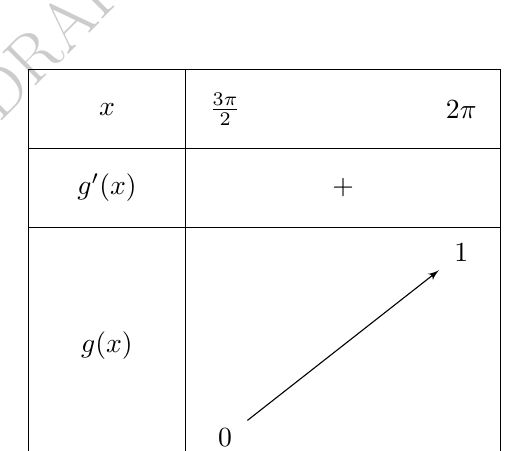
\begin{tikzpicture}
    % Initialisation du tableau
    \tkzTabInit[lgt=2, espcl=3]
    {$x$ /1, $g'(x)$ /1, $g(x)$ /3} 
    {$\frac{3\pi}{2}$, $2\pi$}

    % Ligne de signes de g'(x)
    \tkzTabLine{,+,}
    
    % Ligne de variations de g(x)
    \tkzTabVar{-/$0$, +/$1$,}
\end{tikzpicture}
\end{center}

\end{spacing}
\end{document}
